\documentclass{article}
\usepackage[ngerman]{babel}
\usepackage[utf8]{inputenc}
\usepackage{graphicx}
\usepackage{color}
\usepackage{xcolor}
\usepackage{listings}
\usepackage{comment}
\renewcommand{\lstlistingname}{Auflistung}

\colorlet{punct}{red!60!black}
\definecolor{background}{HTML}{EEEEEE}
\definecolor{delim}{RGB}{20,105,176}
\colorlet{numb}{magenta!60!black}

\lstdefinelanguage{json}{
    basicstyle=\normalfont\ttfamily,
    numbers=left,
    numberstyle=\scriptsize,
    stepnumber=1,
    numbersep=8pt,
    showstringspaces=false,
    breaklines=true,
    frame=lines,
    backgroundcolor=\color{background},
    literate=
     *{0}{{{\color{numb}0}}}{1}
      {1}{{{\color{numb}1}}}{1}
      {2}{{{\color{numb}2}}}{1}
      {3}{{{\color{numb}3}}}{1}
      {4}{{{\color{numb}4}}}{1}
      {5}{{{\color{numb}5}}}{1}
      {6}{{{\color{numb}6}}}{1}
      {7}{{{\color{numb}7}}}{1}
      {8}{{{\color{numb}8}}}{1}
      {9}{{{\color{numb}9}}}{1}
      {:}{{{\color{punct}{:}}}}{1}
      {,}{{{\color{punct}{,}}}}{1}
      {\{}{{{\color{delim}{\{}}}}{1}
      {\}}{{{\color{delim}{\}}}}}{1}
      {[}{{{\color{delim}{[}}}}{1}
      {]}{{{\color{delim}{]}}}}{1},
}

\newcommand*{\signature}[2]{%
    \par\noindent\makebox[2.0in]{\hrulefill} \hfill\makebox[2.0in]{\hrulefill}%
    \par\noindent\makebox[2.0in][l]{Unterschrift #1}      \hfill\makebox[2.0in][l]{Unterschrift #2}%
}%

\newcommand{\blankpage}{
\newpage
\thispagestyle{empty}
\mbox{}
\newpage
}

\setlength{\parindent}{0pt}

\begin{document}
\shorthandoff{"}

\begin{titlepage}
  \topmargin0mm
  \setlength{\parindent}{0em}

\begin{minipage}{\textwidth}
    \centering
    \vspace{0.8cm}
    \begin{large}Hochschule RheinMain\\
    Fachbereich Design Informatik Medien\\
    Studiengang Angewandte Informatik\end{large}
\end{minipage}

\begin{minipage}{\textwidth}
    \centering
    \vspace{0.8cm}
   \begin{large} 
Exposé Bachelor-Arbeit\\
	\end{large} 
    \renewcommand{\baselinestretch}{1}
    \small\normalsize
\end{minipage}
\begin{minipage}{\textwidth}
    \centering
    \vspace{0.8cm}
   \begin{large} 
Titelvorschlag:\\
Entwurf, prototypische Implementierung und Evaluation eines Sicherheitskonzepts für die Authentifizierung und Autorisierung von Fernzugriffen auf eine Automatisierungsanlage
	\end{large}    
    \vspace{4cm}
    \renewcommand{\baselinestretch}{1}
    \small\normalsize
\end{minipage}
\end{titlepage}
\clearpage

\blankpage

\pagenumbering{Roman}
\tableofcontents
\clearpage

\clearpage	
\pagenumbering{arabic}
\pagestyle{plain}

\section{Einleitung}

Die Bachelor-Arbeit soll in der Abteilung Kälte- und Gebäudeleittechnik der Firma Eckelmann durchgeführt werden. Im Bereich Kältetechnik wird Regelungstechnik zur Vernetzung und Überwachung von Kälteanlagen entwickelt. Hierzu gehören die Produkte aus der E*LDS Reihe. Diese beinhalten Verbundsteuerungen zur Kälteerzeugung, Kühlstellenregler zur temperaturgenauen Reglung aller Arten von Kühlmöbeln und Kühlräumen, Funk-Temperatursensoren und der Marktrechner als zentrale Intelligenz einer Kälteanlage. Das Team Datentechnik entwickelt die Software für den Marktrechner und stellt das zu behandelnde Problemfeld. 

\section{Problemfeld}

Der Marktrechner ist das Herzstück einer Kälteanlage. Über einen CAN-Bus ist er mit allen Komponenten der Anlage verbunden. Er ist in der Lage, Komponenten zentral zu parametrieren und zu überwachen. Auf dem internen Speicher werden sämtliche Betriebsdaten und Betriebszustände, Meldungen und Alarme archiviert. Die 24-Stunden Überwachung vor Ort durch einen Mitarbeiter ist bei der Menge an Anlagen nicht wirtschaftlich. Deshalb werden heutzutage Fernservice-Zentralen eingesetzt. Aktuell sind Fernservice-Zentralen über VPN mit einem oder mehreren Unternehmensnetzwerken, ihrer Kunden, verbunden. Über dieses können die Marktrechner erreicht werden. Auf diese Weise kann eine einzige Fernservice-Zentrale Tausende Marktrechner überwachen. Tritt ein Fehler auf, kann die Fernservice-Zentrale einen Mitarbeiter zum betreffenden Kunden schicken, der die Anlage instand setzt.

\begin{comment}
@startuml

package "Unternehmensnetzwerk A" as UA {
  [Marktrechner 1]
  [Marktrechner 2]
  [...]
  [Marktrechner n]
}

package "Unternehmensnetzwerk B" as UB {
}

package "Unternehmensnetzwerk C" as UC {
}

cloud VPN {
}

["Fernservice-Zentrale"] -down- VPN
VPN -down- UA
VPN -left- UB
VPN -right- UC
UA - [Marktrechner n]
UA - [...]
UA - [Marktrechner 2]
UA - [Marktrechner 1]

@enduml
\end{comment}

\begin{figure}[h]
\centering
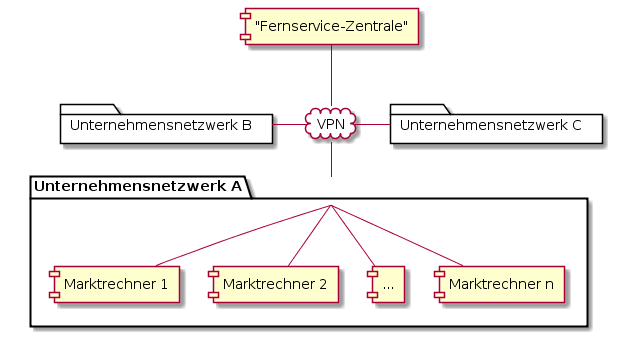
\includegraphics[scale=0.5]{expose_thesis.png}
\caption{Aktuelle Vernetzung}
\label{fig:current_setup}
\end{figure}

Über VPN ist die Kommunikation von der Fernservice-Zentrale bis zum Unternehmensnetzwerk abgesichert. Im Netzwerk des Unternehmens ist der gesamte Datenverkehr zu und von den Marktrechnern allerdings unverschlüsselt. Daten könnten somit von jedem Teilnehmer im Netzwerk mitgelesen werden. Darüber hinaus wäre der Zugriff auf die Daten bei bekannter IP-Adresse möglich, denn es gibt keine geeignete Authentifizierung und Autorisierung. Insbesondere bei Aufrufen zur Systemveränderung kann dies zu Problemen führen. Der aktuelle Zugriff auf die Daten wird über Webservices, auf Basis von einfachen XML-RPCs, realisiert. Im Rahmen des absolvierten Praktikums wurde eine neue Webservice-Schnittstelle geschrieben, welcher das weit verbreitete REST-Konzept für Webanwendungen zu Grunde liegt. Das RestGateway führt zur Zeit keine Authentifizierung und Autorisierung durch. Es wurde aber mit dem Hintergrund entwickelt, diese Funktionen zu integrieren (vgl. Praktikumsbericht).

\section{Ziel der Arbeit}

Ziel der Arbeit ist ein Vergleich zweier Systeme zur Authentifizierung und Autorisierung. Das erste System, CodeMeter der WIBU-SYSTEMS AG, ist spezialisiert auf den Einsatz in Hardwareprodukten, wie dem Marktrechner. Authentifizierung kann hierbei auf der Softwareebene als auch auf Hardwareebene durch WIBU-Hardware geschehen. Das zweite System freeRadius (Network RADIUS Inc.) ist eine reine Open-Source-Softwarelösung und nutzt das Radius-Protokoll.

Die Schwerpunkte des Vergleichs sollen auf Installation, Verwaltung und Distribution von Identifikationsnachweisen liegen. Neben dem Vergleich soll ein Prototyp für eine Marktrechnerkomponente entwickelt werden, der sich gegen eines dieser Systeme authentifiziert und autorisiert. Für diesen Zweck bieten beide Systeme Software-Bibliotheken an.

\section{Methoden}

Vergleich zweier Softwareprodukte, anhand zu definierender Schwerpunkte, durch Literaturarbeit. Prototypische Implementierung der Benutzung eines der Systeme.

\section{Erwartete Ergebnisse}

\begin{itemize}
\item Evaluation anhand definierter Schwerpunkte.
\item Entscheidung, ob sich ein System zum Einsatz eignet? Welches?
\item Prototyp für eine Marktrechnerkomponente.
\end{itemize}

\section{Vorbedingungen}

\begin{itemize}
\item freeRadius: Dokumentation + Software 
\item Radiusclient: Dokumentation + Software
\item CodeMeter: Dokumentation + Software + Hardware
\end{itemize}

\section{Quellen}

The FreeRADIUS Project - http://freeradius.org\\
Radiusclient - http://wiki.freeradius.org/project/Radiusclient\\
WIBU-Systems - CodeMeter - http://www.wibu.com/codemeter.html

\end{document}